\documentclass[usenames,dvipsnames,tikz]{standalone}
\usetikzlibrary{shapes.geometric}
%\usepackage{xcolor}
\colorlet{tBlue}{RoyalBlue!35!Cerulean}
\colorlet{tRed}{Red}
\definecolor{tGreen2}{HTML}{569909}
\definecolor{tOrange}{HTML}{FA7602}
\definecolor{tPurple}{HTML}{7356AF} %tikz color %ECDBFF
%\usepackage{tikz}
%\usepackage{standalone}
%\usepackage{amsmath}
%\usepackage{mathtools}
\begin{document}	
	
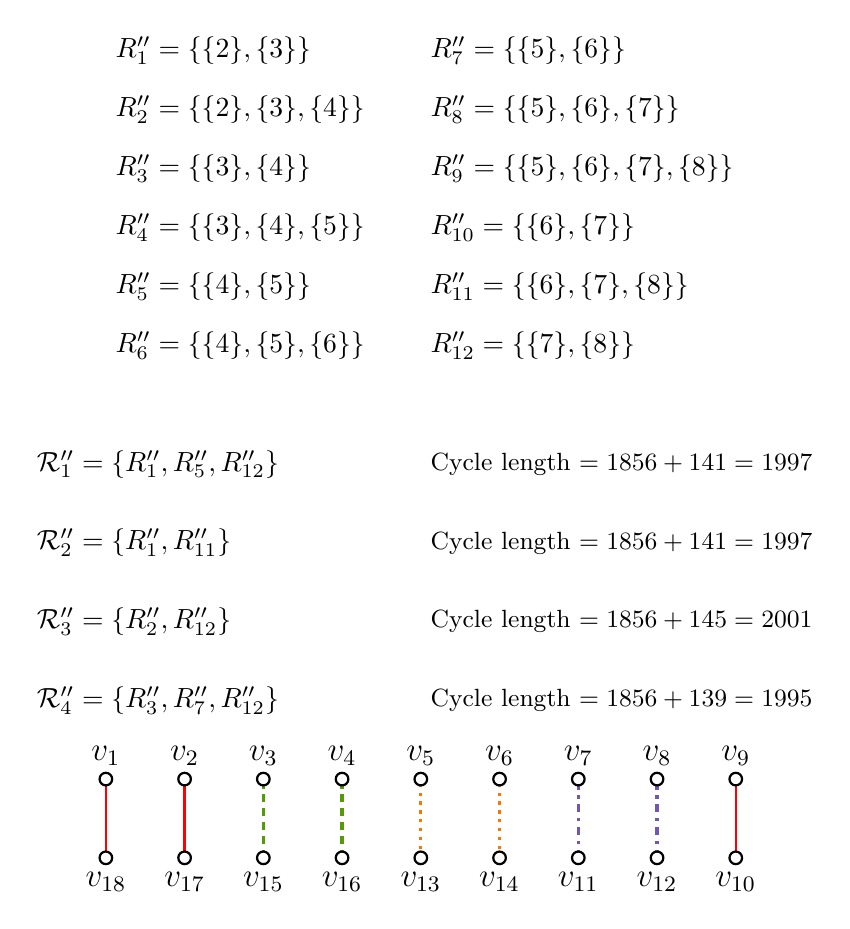
\begin{tikzpicture}
%\draw [help lines] (-1,-1) grid (13, 13);

%% LIST OF EDGES FOR BCR.
%\draw [thick, tRed] (9,7.5) -- (9,8.5);
%\draw [thick, tRed] (10,7.5) -- (10,8.5);
%\draw [thick, tRed] (11,7.5) -- (11,8.5);
%\draw [thick, tRed] (12,7.5) -- (12,8.5);
%\draw [thick, tRed] (13,7.5) -- (13,8.5);
%\draw [thick, tRed] (14,7.5) -- (14,8.5);
%\draw [thick, tRed] (15,7.5) -- (15,8.5);
%\draw [thick, tRed] (16,7.5) -- (16,8.5);
%\draw [thick, tRed] (17,7.5) -- (17,8.5);

%\draw [fill=white, thick] (9,7.5) circle [radius = 0.08];
%\draw [fill=white, thick] (10,7.5) circle [radius = 0.08];
%\draw [fill=white, thick] (11,7.5) circle [radius = 0.08];
%\draw [fill=white, thick] (12,7.5) circle [radius = 0.08];
%\draw [fill=white, thick] (13,7.5) circle [radius = 0.08];
%\draw [fill=white, thick] (14,7.5) circle [radius = 0.08];
%\draw [fill=white, thick] (15,7.5) circle [radius = 0.08];
%\draw [fill=white, thick] (16,7.5) circle [radius = 0.08];
%\draw [fill=white, thick] (17,7.5) circle [radius = 0.08];
%
%\draw [fill=white, thick] (9,8.5) circle [radius = 0.08];
%\draw [fill=white, thick] (10,8.5) circle [radius = 0.08];
%\draw [fill=white, thick] (11,8.5) circle [radius = 0.08];
%\draw [fill=white, thick] (12,8.5) circle [radius = 0.08];
%\draw [fill=white, thick] (13,8.5) circle [radius = 0.08];
%\draw [fill=white, thick] (14,8.5) circle [radius = 0.08];
%\draw [fill=white, thick] (15,8.5) circle [radius = 0.08];
%\draw [fill=white, thick] (16,8.5) circle [radius = 0.08];
%\draw [fill=white, thick] (17,8.5) circle [radius = 0.08];

%\node at (9,7.2) {\large{$v_{18}$}};
%\node at (10,7.2) {\large{$v_{17}$}};
%\node at (11,7.2) {\large{$v_{16}$}};
%\node at (12,7.2) {\large{$v_{15}$}};
%\node at (13,7.2) {\large{$v_{14}$}};
%\node at (14,7.2) {\large{$v_{13}$}};
%\node at (15,7.2) {\large{$v_{12}$}};
%\node at (16,7.2) {\large{$v_{11}$}};
%\node at (17,7.2) {\large{$v_{10}$}};

%\node at (9,8.8) {\large{$v_1$}};
%\node at (10,8.8) {\large{$v_2$}};
%\node at (11,8.8) {\large{$v_3$}};
%\node at (12,8.8) {\large{$v_4$}};
%\node at (13,8.8) {\large{$v_5$}};
%\node at (14,8.8) {\large{$v_6$}};
%\node at (15,8.8) {\large{$v_7$}};
%\node at (16,8.8) {\large{$v_8$}};
%\node at (17,8.8) {\large{$v_9$}};

%\node at (9,6.7) {$C_1$};
%\node at (10,6.7) {$C_1$};
%\node at (11,6.7) {$C_2$};
%\node at (12,6.7) {$C_3$};
%\node at (13,6.7) {$C_1$};
%\node at (14,6.7) {$C_2$};
%\node at (15,6.7) {$C_3$};
%\node at (16,6.7) {$C_4$};
%\node at (17,6.7) {$C_4$};

%---------------------------------------
% Edge subsets old
%\node [right] at (0.75,10.25) {$R''_1 = \{\{v_2, v_{17}\}, \{v_3, v_{16}\}\}$};
%\node [right] at (0.75,9.5) {$R''_2 = \{\{v_2, v_{17}\}, \{v_3, v_{16}\}, \{v_4, v_{15}\}\}$};
%\node [right] at (0.75,8.75) {$R''_3 = \{\{v_3, v_{16}\}, \{v_4, v_{15}\}\}$};
%\node [right] at (0.75,8) {$R''_4 = \{\{v_3, v_{16}\}, \{v_4, v_{15}\}, \{v_5, v_{14}\}\}$};
%\node [right] at (0.75,7.25) {$R''_5 = \{\{v_4, v_{15}\}, \{v_5, v_{14}\}\}$};
%\node [right] at (0.75,6.5) {$R''_6 = \{\{v_4, v_{15}\}, \{v_5, v_{14}\}, \{v_6, v_{13}\}\}$};
%
%\node [right] at (7,10.25) {$R''_7 = \{\{v_5, v_{14}\}, \{v_6, v_{13}\}\}$};
%\node [right] at (7,9.5) {$R''_8 = \{\{v_5, v_{14}\}, \{v_6, v_{13}\}, \{v_7, v_{12}\}\}$};
%\node [right] at (7,8.75) {$R''_9 = \{\{v_5, v_{14}\}, \{v_6, v_{13}\}, \{v_7, v_{12}\}, \{v_8, v_{11}\}\}$};
%\node [right] at (7,8) {$R''_{10} = \{\{v_6, v_{13}\}, \{v_7, v_{12}\}\}$};
%\node [right] at (7,7.25) {$R''_{11} = \{\{v_6, v_{13}\}, \{v_7, v_{12}\}, \{v_8, v_{11}\}\}$};
%\node [right] at (7,6.5) {$R''_{12} = \{\{v_7, v_{12}\}, \{v_8, v_{11}\}\}$};

%---------------------------------------
% Edge subsets
\node [right] at (1,10.25) {$R''_1 = \{\{2\}, \{3\}\}$};
\node [right] at (1,9.5) {$R''_2 = \{\{2\}, \{3\}, \{4\}\}$};
\node [right] at (1,8.75) {$R''_3 = \{\{3\}, \{4\}\}$};
\node [right] at (1,8) {$R''_4 = \{\{3\}, \{4\}, \{5\}\}$};
\node [right] at (1,7.25) {$R''_5 = \{\{4\}, \{5\}\}$};
\node [right] at (1,6.5) {$R''_6 = \{\{4\}, \{5\}, \{6\}\}$};

\node [right] at (5,10.25) {$R''_7 = \{\{5\}, \{6\}\}$};
\node [right] at (5,9.5) {$R''_8 = \{\{5\}, \{6\}, \{7\}\}$};
\node [right] at (5,8.75) {$R''_9 = \{\{5\}, \{6\}, \{7\}, \{8\}\}$};
\node [right] at (5,8) {$R''_{10} = \{\{6\}, \{7\}\}$};
\node [right] at (5,7.25) {$R''_{11} = \{\{6\}, \{7\}, \{8\}\}$};
\node [right] at (5,6.5) {$R''_{12} = \{\{7\}, \{8\}\}$};


%---------------------------------------

% Collections
\node [right] at (0,5) {$\mathcal{R}''_1 = \{R''_1, R''_5, R''_{12}\}$};
%\node [right] at (5,5) {$w(\mathcal{R}''_1) = 141$};
\node [right] at (5, 5) {\small{Cycle length $=1856 + 141 = 1997$}};

\node [right] at (0,4) {$\mathcal{R}''_2 = \{R''_1, R''_{11}\}$};
%\node [right] at (5,4) {$w(\mathcal{R}''_2) = 141$};
\node [right] at (5,4) {\small{Cycle length $=1856 + 141 = 1997$}};

\node [right] at (0,3) {$\mathcal{R}''_3 = \{R''_2, R''_{12}\}$};
%\node [right] at (5,3) {$w(\mathcal{R}''_3) = 145$};
\node [right] at (5,3) {\small{Cycle length $=1856 + 145 = 2001$}};

\node [right] at (0,2) {$\mathcal{R}''_4 = \{R''_3, R''_7, R''_{12}\}$};
%\node [right] at (5,2) {$w(\mathcal{R}''_4) = 139$};
\node [right] at (5,2) {\small{Cycle length $=1856 + 139 = 1995$}};

%--------------------------------------
% New set of edges R'
\draw [thick, tRed] (1,0) -- (1,1);
\draw [thick, tRed] (2,0) -- (2,1);
\draw [very thick, densely dashed, tGreen2] (3,0) -- (3,1);
\draw [very thick, densely dashed, tGreen2] (4,0) -- (4,1);
\draw [very thick, dotted, tOrange] (5,0) -- (5,1);
\draw [very thick, dotted, tOrange] (6,0) -- (6,1);
\draw [very thick, dash dot, tPurple] (7,0) -- (7,1);
\draw [very thick, dash dot, tPurple] (8,0) -- (8,1);
\draw [thick, tRed] (9,0) -- (9,1);

%\draw [thick, tRed] (3.375,0) -- (3.375,1);
%\draw [thick, tRed] (4.375,0) -- (4.375,1);
%\draw [very thick, densely dashed, tGreen2] (5.375,0) -- (5.375,1);
%\draw [very thick, densely dashed, tGreen2] (6.375,0) -- (6.375,1);
%\draw [very thick, dotted, tOrange] (7.375,0) -- (7.375,1);
%\draw [very thick, dotted, tOrange] (8.375,0) -- (8.375,1);
%\draw [very thick, dash dot, tPurple] (9.375,0) -- (9.375,1);
%\draw [very thick, dash dot, tPurple] (10.375,0) -- (10.375,1);
%\draw [thick, tRed] (11.375,0) -- (11.375,1);

\draw [fill=white, thick] (1,0) circle [radius = 0.08];
\draw [fill=white, thick] (2,0) circle [radius = 0.08];
\draw [fill=white, thick] (3,0) circle [radius = 0.08];
\draw [fill=white, thick] (4,0) circle [radius = 0.08];
\draw [fill=white, thick] (5,0) circle [radius = 0.08];
\draw [fill=white, thick] (6,0) circle [radius = 0.08];
\draw [fill=white, thick] (7,0) circle [radius = 0.08];
\draw [fill=white, thick] (8,0) circle [radius = 0.08];
\draw [fill=white, thick] (9,0) circle [radius = 0.08];

\draw [fill=white, thick] (1,1) circle [radius = 0.08];
\draw [fill=white, thick] (2,1) circle [radius = 0.08];
\draw [fill=white, thick] (3,1) circle [radius = 0.08];
\draw [fill=white, thick] (4,1) circle [radius = 0.08];
\draw [fill=white, thick] (5,1) circle [radius = 0.08];
\draw [fill=white, thick] (6,1) circle [radius = 0.08];
\draw [fill=white, thick] (7,1) circle [radius = 0.08];
\draw [fill=white, thick] (8,1) circle [radius = 0.08];
\draw [fill=white, thick] (9,1) circle [radius = 0.08];

%\draw [fill=white, thick] (3.375,0) circle [radius = 0.08];
%\draw [fill=white, thick] (4.375,0) circle [radius = 0.08];
%\draw [fill=white, thick] (5.375,0) circle [radius = 0.08];
%\draw [fill=white, thick] (6.375,0) circle [radius = 0.08];
%\draw [fill=white, thick] (7.375,0) circle [radius = 0.08];
%\draw [fill=white, thick] (8.375,0) circle [radius = 0.08];
%\draw [fill=white, thick] (9.375,0) circle [radius = 0.08];
%\draw [fill=white, thick] (10.375,0) circle [radius = 0.08];
%\draw [fill=white, thick] (11.375,0) circle [radius = 0.08];
%
%\draw [fill=white, thick] (3.375,1) circle [radius = 0.08];
%\draw [fill=white, thick] (4.375,1) circle [radius = 0.08];
%\draw [fill=white, thick] (5.375,1) circle [radius = 0.08];
%\draw [fill=white, thick] (6.375,1) circle [radius = 0.08];
%\draw [fill=white, thick] (7.375,1) circle [radius = 0.08];
%\draw [fill=white, thick] (8.375,1) circle [radius = 0.08];
%\draw [fill=white, thick] (9.375,1) circle [radius = 0.08];
%\draw [fill=white, thick] (10.375,1) circle [radius = 0.08];
%\draw [fill=white, thick] (11.375,1) circle [radius = 0.08];

\node at (1,-0.3) {\large{$v_{18}$}};
\node at (2,-0.3) {\large{$v_{17}$}};
\node at (3,-0.3) {\large{$v_{15}$}};
\node at (4,-0.3) {\large{$v_{16}$}};
\node at (5,-0.3) {\large{$v_{13}$}};
\node at (6,-0.3) {\large{$v_{14}$}};
\node at (7,-0.3) {\large{$v_{11}$}};
\node at (8,-0.3) {\large{$v_{12}$}};
\node at (9,-0.3) {\large{$v_{10}$}};

\node at (1,1.3) {\large{$v_1$}};
\node at (2,1.3) {\large{$v_2$}};
\node at (3,1.3) {\large{$v_3$}};
\node at (4,1.3) {\large{$v_4$}};
\node at (5,1.3) {\large{$v_5$}};
\node at (6,1.3) {\large{$v_6$}};
\node at (7,1.3) {\large{$v_7$}};
\node at (8,1.3) {\large{$v_8$}};
\node at (9,1.3) {\large{$v_9$}};

%\node at (3.375,-0.3) {\large{$v_{18}$}};
%\node at (4.375,-0.3) {\large{$v_{17}$}};
%\node at (5.375,-0.3) {\large{$v_{15}$}};
%\node at (6.375,-0.3) {\large{$v_{16}$}};
%\node at (7.375,-0.3) {\large{$v_{13}$}};
%\node at (8.375,-0.3) {\large{$v_{14}$}};
%\node at (9.375,-0.3) {\large{$v_{11}$}};
%\node at (10.375,-0.3) {\large{$v_{12}$}};
%\node at (11.375,-0.3) {\large{$v_{10}$}};
%
%\node at (3.375,1.3) {\large{$v_1$}};
%\node at (4.375,1.3) {\large{$v_2$}};
%\node at (5.375,1.3) {\large{$v_3$}};
%\node at (6.375,1.3) {\large{$v_4$}};
%\node at (7.375,1.3) {\large{$v_5$}};
%\node at (8.375,1.3) {\large{$v_6$}};
%\node at (9.375,1.3) {\large{$v_7$}};
%\node at (10.375,1.3) {\large{$v_8$}};
%\node at (11.375,1.3) {\large{$v_9$}};




\end{tikzpicture}
	
\end{document}